\capitulo{5}{Aspectos relevantes del desarrollo del proyecto}

\section{\textit{Navigation Mesh}} \label{referenciaNavMesh}
Una \textit{Navigation Mesh} o \textit{Nav Mesh} es un conjunto de polígonos, triángulos normalmente, que se usan en los motores gráficos 3D para representar la zona o camino recorrible de un agente. Se crean a partir de los objetos estáticos de una escena, que son los obstáculos, donde no se puede desplazar. El resto de la zona de la escena será zona recorrible por donde nos podemos desplazar.

En relación por ejemplo al \Astar, sería el equivalente a la matriz que representa el mapa donde se buscará los nodos a explorar.

Está formada por los vértices de los polígonos, y si un punto está dentro del área que forman, entonces ese punto es recorrible. Esto es mas realista en un escenario en tres dimensiones, como los representados por los motores 3D, debido a que permite un movimiento menos discretizado, al contrario que las cuadrículas de casillas que se adecuan más a una representación en dos dimensiones. Y si consideramos los vértices los nodos sucesores, resulta más óptimo computacionalmente, ya que el número de nodos (vértices) a explorar es menor, debido a que no tenemos que tener en cuenta todos los puntos intermedios hasta llegar al vértice, si no únicamente si el vértice es visible o alcanzable desde el nodo actual.

Hemos usado una \textit{Nav Mesh} para generar de forma automática el mapa para el \Astar. En \textit{Unity} esto se puede hacer de dos formas. En versiones anteriores a la versión 5.6 solo es posible generarlo desde el editor antes del tiempo de ejecución. A partir de la versión 5.6, que permite acceder a las herramientas del editor en tiempo de ejecución, se puede construir a través de \textit{NavMeshBuilder}, dando mucha más libertad a la hora de crear mapas de forma dinámica o interactiva. Lamentablemente, no se pudo usar la versión 5.6 y la versión más actual que funcionaba en el equipo de desarrollo fue la 5.3.6.

\begin{figure}[htpb]
    \centering
    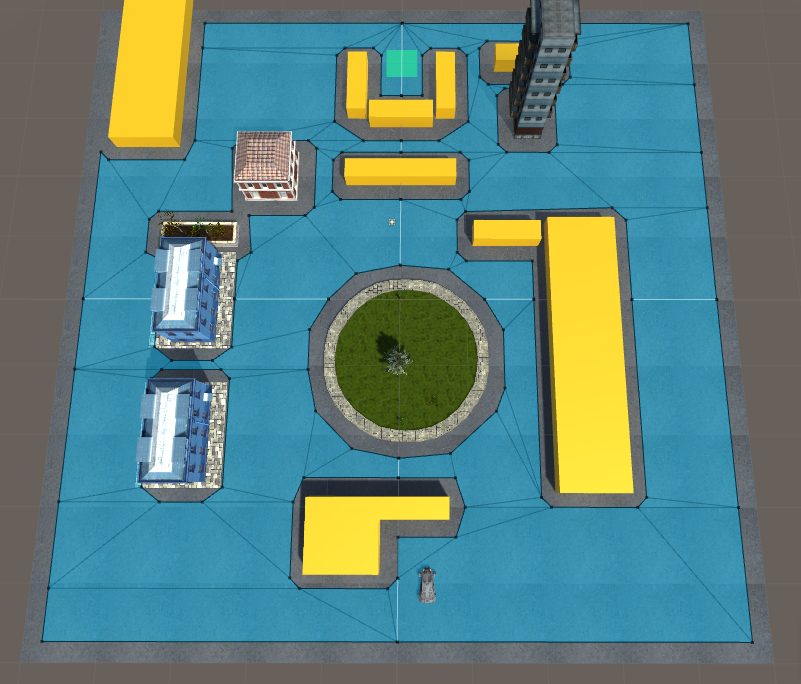
\includegraphics[width=\textwidth,height=10cm,keepaspectratio=true]{nav_mesh}
    \caption[Imagen de un \textit{Nav Mesh} en \textit{Unity}]{Imagen de un \textit{Nav Mesh} en \textit{Unity}.}
    \label{fig:basics AFM sketch}
\end{figure}

La clase \textit{NavMesh} de \textit{Unity} tiene métodos que podemos usar como \textit{RayTrace}, que lanza un rayo desde un vector a otro y devuelve si son visibles dentro de la \textit{NavMesh}, es decir, si existe una línea recta entre ellos que los una dentro del camino recorrible. Este método lo hemos usado para decidir si un nodo sucesor es válido o no. Al usarlo encontramos un \textit{bug} que producía que a veces no se encontrará el camino o bucles infinitos al recorrer las listas. Esto es debido a que puede ocurrir que no devuelva lo mismo dependiendo del orden o sentido en el que se le indiquen los vectores entre los que lanzar el rayo. Por ejemplo \textit{RayTrace}(vector1, vector2) puede ser visible pero \textit{RayTrace}(vector2, vector1) no. Para solucionarlo, tuvimos que vigilar el orden con el que recorríamos las listas, y decidimos, que cuando fuera posible, comprobar que para que fuera un sucesor válido debe ser visible en los dos sentidos.

\section{Cola de prioridad}
Uno de los problemas que se encontraron al usar C\# y en concreto la versión que utiliza \textit{Unity} ha sido el no poder usar todos las estructuras de datos de C\# y que algunas estructuras de datos no estaban disponibles directamente en C\#.

Una de estas estructuras de datos que no se encuentran en C\# es la cola de prioridad. La cola de prioridad es utilizada por el \Astar para almacenar los estados que se van a explorar. Se ordenan según su coste y se extrae de la cola aquel que tenga menos coste para ser el siguiente en ser explorado.

Para tener acceso a una cola de prioridad hemos usado
\textit{High Speed Priority Queue for C\#\cite{bluerajacola}}\footnote{\url{https://github.com/BlueRaja/High-Speed-Priority-Queue-for-C-Sharp}}.

Los motivos para utilizarla han sido que tiene una licencia MIT que permite usarla libremente. Es sencilla y fácil de usar, además está creada con el objetivo de ser usada para \textit{Path Finding} con lo que encaja en los objetivos del proyecto.

\section{Física del vehículo}
\textit{Unity} dispone de un motor de físicas integrado basado en el \textit{PhysX} de \textit{Nvidia}\footnote{\url{https://blogs.unity3d.com/es/2014/07/08/high-performance-physics-in-unity-5/}}. Una de las características que se encuentran en el motor de físicas y que han resultado de gran utilidad para la realización del proyecto han sido los \textit{Wheel Colliders}

\begin{figure}[htpb]
    \centering
    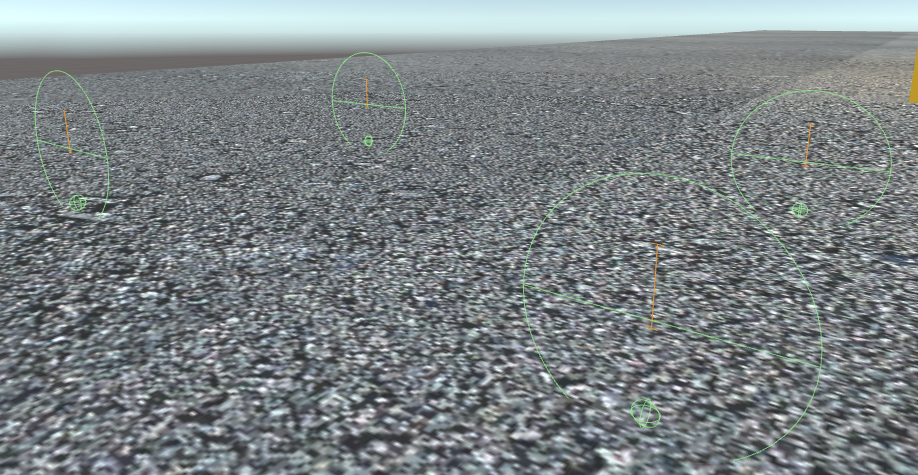
\includegraphics[width=\textwidth,height=10cm,keepaspectratio=true]{wheelcolliders}
    \caption[Representación de los \textit{Wheel Colliders} en \textit{Unity}]{Representación de los cuatro \textit{Wheel Colliders} en \textit{Unity}.}
    \label{fig:basics AFM sketch}
\end{figure}

Los \textit{Wheel Colliders} son una simulación realista de las ruedas de un vehículo y permiten simular todas la físicas necesarias para el vehículo. Tienen tanto simulación del giro de las ruedas como de la fuerza que aplica el motor a las mismas, y una simulación del freno, además de otras simulaciones como la amortiguación que no se han controlado de forma directa en este proyecto.

El uso de los \textit{Wheel Colliders} nos ha permitido la simulación realista de un vehículo con tracción a las cuatro ruedas y un radio de giro de las mismas de 45 grados. Su uso es independiente del modelo del vehículo usado, pudiendo adaptarlo a cualquier modelo cambiando sus parámetros. Tampoco hay limitaciones al número de \textit{Wheel Colliders} que podemos usar, de tal forma que es posible simular una motocicleta, un camión o cualquier otro vehículo que use ruedas.

\section{Modelos utilizados}
Los modelos usados han sido los que estaban disponibles en la \textit{Assets Store}\footnote{\url{https://www.assetstore.unity3d.com/}} de \textit{Unity}.

Principalmente hemos usado los \textit{Standard Assets 1.1.2}\footnote{\url{https://www.assetstore.unity3d.com/en/\#!/content/32351}} de \textit{Unity} de donde hemos utilizado el modelo del coche, y cuyos ejemplos nos han servido para aprender como usar \textit{Unity}.

El siguiente conjunto de \textit{assets} que más hemos utilizado ha sido \textit{Low Poly Street Pack 1.0}\footnote{\url{https://www.assetstore.unity3d.com/en/\#!/content/67475}} de \textit{Dynamic Art}, de donde hemos usado la mayor parte de los edificios y elementos del escenario.

En menor medida también se han utilizado elementos de \textit{Abandoned Building 1.0}\footnote{\url{https://www.assetstore.unity3d.com/en/\#!/content/62875}} de Aleksey Kozhemyakim, \textit{Block Building Pack 1.0}\footnote{\url{https://www.assetstore.unity3d.com/en/\#!/content/13925}} de CGY (Yemelyan K.), \textit{Building Apartment 1.0}\footnote{\url{https://www.assetstore.unity3d.com/en/\#!/content/80004}} de LowlyPoly, \textit{San Francisco House 1.0}\footnote{\url{https://www.assetstore.unity3d.com/en/\#!/content/16640}} de Bretwalda Games, \textit{UK Terraced House Pack 1.0}\footnote{\url{https://www.assetstore.unity3d.com/en/\#!/content/63481}} de rik4000.

Los \textit{assets} usados son gratuitos y siguen la licencia de la \textit{Unity Store}\footnote{\url{https://unity3d.com/es/legal/as_terms}} en el que su uso es libre dentro de juegos y de medios interactivos.

\section{Comparativa de los algoritmos}\label{comparativaAlgoritmos}

En esta sección vamos a comparar los algoritmos dependiendo de si utilizan una representación del espacio de búsqueda continua o discreta. A continuación también compararemos el rendimiento de los distintos algoritmos tomando como referencia al \Astar.

En la tabla 5.1 comparamos los algoritmos teniendo en cuenta como representan el espacio de búsqueda y que limitaciones tienen en cuenta. Podemos observar que el \textit{Hybrid \Astar} es el único que tiene en cuenta el modelo físico de los vehículos, y con ello el único que busca rutas válidas para la mayoría de los casos con vehículos no holonómicos. Además, debido a esto, es el único que puede buscar rutas que indiquen al vehículo a moverse en varios sentidos según su dirección. El resto de algoritmos realizan la búsqueda para vehículos holonómicos no teniendo en cuenta estás restricciones.

\tablaSmall{Comparación de los algoritmos según su representación}{l c c c c }{comparativadiscretocontinuo}
{ \multicolumn{1}{l}{Algoritmo} & Discreto & Continuo & Modelo Físico & Varios Sentidos \\}{ 
\Astar & X & & &\\
Theta* & X & & & \\
\Astar vértices & & X & &\\
Hybrid \Astar & & X & X & X \\
}

En la tabla 5.2 comparamos el rendimiento de los algoritmos usados en las mismas condiciones y buscando una ruta con los mismo inicio y meta. Hemos tomado el \Astar como referencia ya que el resto se basan en el. Los resultados son los esperados. El Theta* es más lento debido a los cálculos extra que debe hacer para comprobar si puede asignar un nodo anterior al nodo sucesor. La versión del \Astar con vértices es mucho más rápida debido a que el número de estados a explorar es mucho menor, al usar los vértices del \textit{Nav Mesh}. El \textit{Hybrid \Astar}, aunque es el que más cálculos debe llevar a cabo, es más rápido debido a la heurística mejorada \ref{hueristicahybrid} que le hemos incluido, donde tiene precalculado el coste desde todos los estados posibles hasta la meta teniendo en cuenta los obstáculos.

\tablaSmall{Comparación de los algoritmos según su rendimiento}{l c c }{comparativarendimiento}
{ \multicolumn{1}{l}{Algoritmo} & Segundos & Porcentaje \\}{ 
\Astar & 6.6 & 100\%\\
Theta* & 10.2 & 155.5\%\\
\Astar vértices & 2.05 & 31.1\%\\
Hybrid \Astar & 4.01 & 60.8\%\\
}
